\chapter{ACID Test Suite}
\label{sec:acid-test-suite}

\newcommand{\bl}[1]{\textcolor{blue}{#1}}
\newcommand{\rd}[1]{\textcolor{red}{#1}}
\newcommand{\gn}[1]{\textcolor{green}{#1}}
\newcommand{\gy}[1]{\textcolor{grey}{\textit{#1}}}

\newcommand{\level}[1]{\textsf{#1}}
\newcommand{\anomaly}[1]{\rd{#1}}
\newcommand{\anolong}[1]{\emph{\rd{#1}}}
\newcommand{\tx}[1]{#1}

\newcommand{\cmark}{\ding{51}}
\newcommand{\xmark}{\ding{55}}


\begin{quote}
  \textit{This chapter is based on the TPCTC~2020 paper ``Towards Testing ACID Compliance in the LDBC Social Network Benchmark''~\cite{DBLP:conf/tpctc/WaudbySKMBS20}, co-authored by several members of the SNB task force.}

  \textit{The framework and reference implementations of the ACID test suite are available at \url{https://github.com/ldbc/ldbc_acid}.}
\end{quote}

Verifying ACID compliance is an important step in the benchmarking process for enabling fair comparison between systems.
The performance benefits of operating with weaker safety guarantees are well established~\cite{DBLP:conf/ds/GrayLPT76} but this can come at the cost of application correctness.
To enable apples vs. apples performance comparisons between systems it is expected they uphold the ACID properties.
Currently, LDBC provides no mechanism for validating ACID compliance within the SNB Interactive workflow.
A simple solution would be to outsource the responsibility of demonstrating ACID compliance to benchmark implementors.
However, the safety properties claimed by a system often do not match observable behaviour~\cite{kingsbury}.
%which could cast doubt on any performance results obtained from SNB Interactive.
To mitigate this problem, benchmarks such as \mbox{TPC-C}~\cite{tpcc} include a number of ACID tests to be executed as part of the benchmarking auditing process.
However, we found these tests cannot readily be applied to our context, as they assume lock-based concurrency control and an interactive query API that provides clients with explicit control over a transaction's lifecyle.
Modern data systems often use optimistic concurrency control mechanisms~\cite{DBLP:journals/sigmod/PavloA16} and offer a restricted query API, such as only executing transactions as stored procedures~\cite{DBLP:conf/vldb/StonebrakerMAHHH07}.
Further, tests that trigger and test row-level locking phenomena, for instance, do not readily map on graph database systems.
Lastly, we found these tests are limited in the range of isolation anomalies they cover.
% TPC-C tests for protection against \anolong{Dirty Writes}, \anolong{Dirty Reads}, \anolong{Fuzzy Reads} and \anolong{Phantoms}.
% Modern databases are often multi-version systems and use optimistic concurrency control mechanisms (based on validation or timestamps)~\cite{DBLP:journals/sigmod/PavloA16} and perform all transaction logic on the server-side or executing transactions as stored procedures~\cite{DBLP:conf/vldb/StonebrakerMAHHH07}
% Moreover, these tests are specifically limited in the range of transactional isolation anomalies they test for.
% \emph{``For conventional locking schemes, isolation should be tested as described. Systems that implement other isolation schemes may require different validation techniques.''}.

This chapter presents the design of an implementation-agnostic ACID-compliance test suite for the Interactive workload\footnote{We acknowledge verifying ACID-compliance with a finite set of tests is not possible. However, the goal is not an exhaustive quality assurance test of a system's safety properties but rather to demonstrate that ACID guarantees are supported.}.
Our guiding design principle was to be agnostic of system-level implementation details, relying solely on client observations to determine the occurrence of non-transactional behaviour.
Thus all systems can be subjected to the same tests and fair comparisons between SNB Interactive performance results can be drawn.
Tests are described in the context of a graph database employing the property graph data model~\cite{DBLP:journals/csur/AnglesABHRV17}.
Reference implementations are given in Cypher~\cite{DBLP:conf/sigmod/FrancisGGLLMPRS18}, the \emph{de facto} standard graph query language.

Particular emphasis is given to testing isolation, covering 10~known anomalies including recently discovered anomalies such as \anolong{Observed Transaction Vanishes}~\cite{DBLP:journals/pvldb/BailisDFGHS13} and \anolong{Fractured Reads}~\cite{DBLP:journals/tods/BailisFGHS16}.
The test suite has been implemented for 5~database systems.\footnote{Available at \url{https://github.com/ldbc/ldbc_acid}.}
A conscious decision was made to keep tests relatively lightweight, as to not add significant overhead to the benchmarking process.

\section{Background}

The tests presented in this chapter are defined on a small core of LDBC SNB schema (extended with properties for versioning) given in \autoref{fig:core-schema}.

\begin{figure}
  \centering
  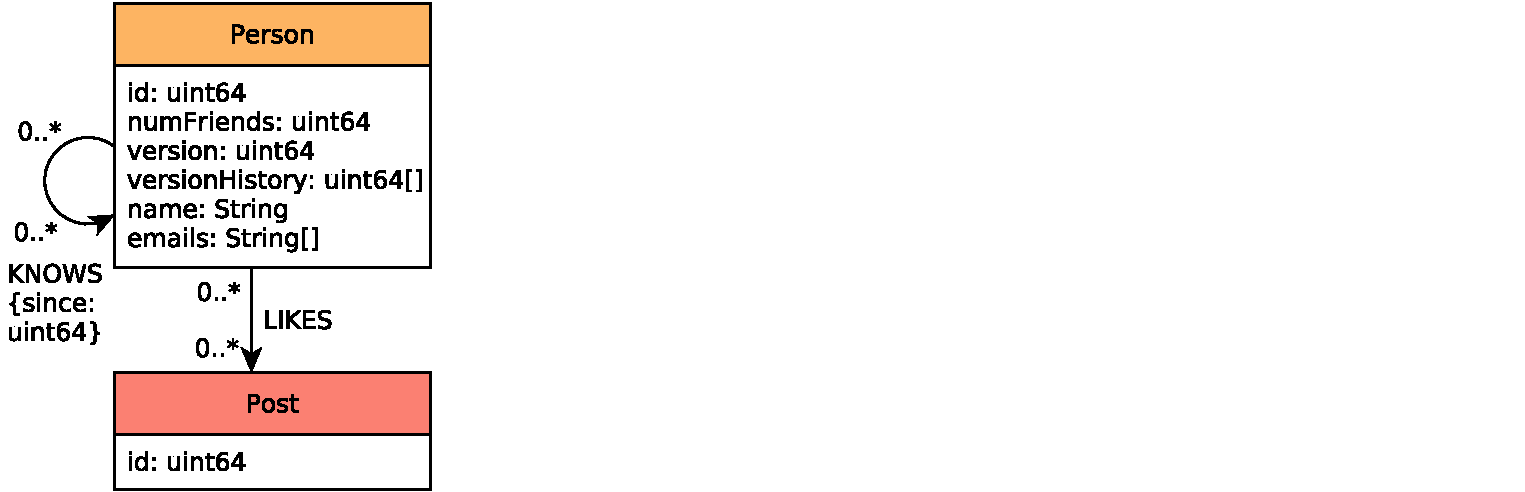
\includegraphics[scale=\yedscale]{figures/acid/core-schema}
  \caption{Graph schema for the ACID test queries.}
  \label{fig:core-schema}
\end{figure}

\begin{figure}
  \centering
  \scriptsize
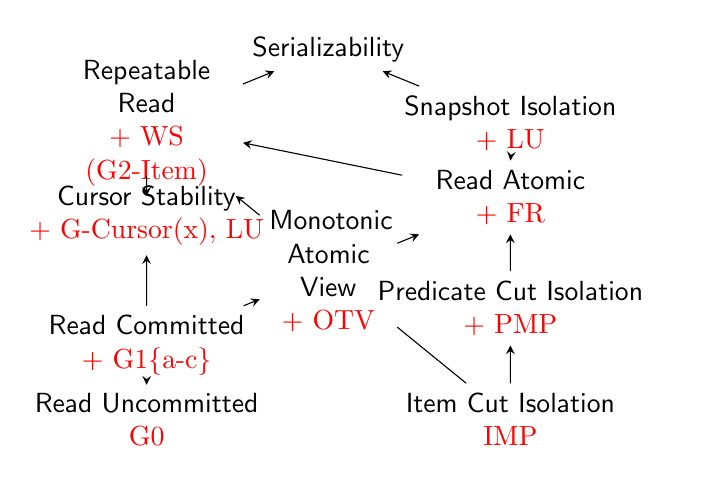
\begin{tikzpicture}[xscale=0.77,yscale=0.47,trim left=0.8cm]
%\draw[help lines] (0,0) grid (12,18);
\node[text width=4cm,align=center] (RU) at (3,1) {
\level{Read Uncommitted}  \\
\anomaly{G0}
};

\node[text width=4cm,align=center] (RC) at (3,3) {
\level{Read Committed}  \\
\anomaly{+ G1\{a-c\}}
};

\node[text width=4cm,align=center] (ICI) at (9,1) {
\level{Item Cut Isolation}  \\
\anomaly{IMP}
};

\node[text width=4cm,align=center] (PCI) at (9,4) {
\level{Predicate Cut Isolation}  \\
\anomaly{+ PMP}
};

\node[text width=1.5cm,align=center] (MAV) at (6,5) {
\level{Monotonic Atomic View}  \\
\anomaly{+ OTV}
};
% we place MAV below Adya’s PL-2L

\node[text width=4cm,align=center] (CS) at (3,6.5) {
\level{Cursor Stability}  \\
\anomaly{+ G-Cursor(x), LU}
};

\node[text width=2.5cm,align=center] (RA) at (9,7) {
\level{Read Atomic}  \\
\anomaly{+ FR}
};

\node[text width=3.3cm,align=center] (SI) at (9,9) {
\level{Snapshot Isolation}  \\
\anomaly{+ LU}
};

\node[text width=2.2cm,align=center] (RR) at (3,9) {
\level{Repeatable Read}  \\
\anomaly{+ WS (G2-Item)}
}; % Adya's

\node[text width=4cm,align=center] (S) at (6,11) {
  \level{Serializability}
};

\draw [->,>=stealth] (RU) -- (RC);
\draw [->,>=stealth] (ICI) -- (PCI);
\draw [->,>=stealth] (RC) -- (MAV);
% \draw [->,>=stealth,postaction={-,draw=white,dash pattern=on 0pt off 3cm on 3cm off 3cm}] (ICI) -- (RR);
\draw (ICI) -- (MAV);
\draw [->,>=stealth] (MAV) -- (RR);
\draw [->,>=stealth] (PCI) -- (RA);
\draw [->,>=stealth] (MAV) -- (RA);
\draw [->,>=stealth] (RA) -- (RR);
\draw [->,>=stealth] (RA) -- (SI);
\draw [->,>=stealth] (SI) -- (S);
\draw [->,>=stealth] (RR) -- (S);
\draw [->,>=stealth] (CS) -- (RR);
\draw [->,>=stealth] (RC) -- (CS);

\end{tikzpicture}
\caption{Hierarchy of isolation levels as described in~\cite{DBLP:journals/tods/BailisFGHS16}. All anomalies are covered except \anomaly{G-Cursor(x)}.}
\label{fig:isolation}

\end{figure}

\section{Atomicity}
\label{sec:atomicity}

\emph{Atomicity} ensures that either all of a transaction's actions are performed, or none are.
Two atomicity tests have been developed.
\textbf{Atomicity-C} checks for every successful commit message a client receives that any data items inserted or modified are subsequently visible.
\textbf{Atomicity-RB} checks for every aborted transaction that all its modifications are not visible.
%
Tests are executed as follows:
(i) load a graph of \texttt{Person} nodes (\autoref{fig:ainitial}) each with a unique \texttt{id} and a set of \texttt{emails};
(ii) a client executes a full graph scan counting the number of nodes, edges and emails (\autoref{fig:acheck}) using the result to initialize a counter \texttt{committed};
(iii) $N$ transaction instances (\autoref{fig:ac}, \autoref{fig:arb}) of the required test are then executed, \texttt{committed} is incremented for each successful commit;
(iii) repeat the full graph scan, storing the result in the variable \texttt{finalState};
(iv) perform the anomaly check: \texttt{committed=finalState}.

The \textbf{Atomicity-C} transaction (\autoref{fig:ac}) randomly selects a \texttt{Person}, creates a new \texttt{Person}, inserts a \texttt{KNOWS} edge and appends an \texttt{email}. The \textbf{Atomicity-RB} transaction (\autoref{fig:arb}) randomly selects a \texttt{Person}, appends an \texttt{email} and attempts to insert a \texttt{Person} only if it does not exist.
Note, for \textbf{Atomicity-RB} if the query API does not offer a \texttt{ROLLBACK} statement constraints such as node uniqueness can be utilized to trigger an abort.

\begin{figure}[htb]
\centering

\begin{lstlisting}[language=cypher,label=fig:ainitial,caption=Cypher query for creating initial data for the \tx{Atomicity} transactions.]
CREATE (:Person {id: 1, name: 'Alice', emails: ['alice@aol.com']}),
       (:Person {id: 2, name: 'Bob', emails: ['bob@hotmail.com', 'bobby@yahoo.com']})
\end{lstlisting}

\begin{minipage}{0.41\linewidth}
\begin{lstlisting}[language=cypher,label=fig:ac,caption=\tx{Atomicity-C Tx.}]
<<BEGIN>>
MATCH (p1:Person {id: $person1Id})
CREATE (p1)-[k:KNOWS]->(p2:Person)
SET
  p1.emails = p1.emails + [$newEmail],
  p2.id = $person2Id,
  k.creationDate = $creationDate
<<COMMIT>>
\end{lstlisting}
\end{minipage}
\quad
\begin{minipage}{0.52\linewidth}
\begin{lstlisting}[language=cypher,label=fig:arb,caption=\tx{Atomicity-RB Tx.}]
<<BEGIN>>
MATCH (p1:Person {id: $person1Id})
SET p1.emails = p1.emails + [$newEmail]
<<IF>> MATCH (p2:Person {id: $person2Id}) exists
<<THEN>> <<ABORT>> <<ELSE>>
CREATE (p2:Person {id: $person2Id, emails: []})
<<END>>
<<COMMIT>>
\end{lstlisting}
\end{minipage}

\begin{lstlisting}[language=cypher,label=fig:acheck,caption=\tx{Atomicity-C/Atomicity-RB:} counting entities in the graph.]
MATCH (p:Person)
RETURN count(p) AS numPersons, count(p.name) AS numNames, sum(size(p.emails)) AS numEmails
\end{lstlisting}
\end{figure}

\section{Isolation}
\label{sec:isolation}

The gold standard isolation level is \level{Serializability}, which offers protection against all possible \emph{anomalies} that can occur from the concurrent execution of transactions.
Anomalies are occurrences of non-serializable behaviour.
Providing \level{Serializability} can be detrimental to performance~\cite{DBLP:conf/ds/GrayLPT76}.
Thus systems offer numerous weak isolation levels such as \level{Read Committed} and \level{Snapshot Isolation} that allow a higher degree of concurrency at the cost of potential non-serializable behaviour.
As such, isolation levels are defined in terms of the anomalies they prevent~\cite{DBLP:conf/ds/GrayLPT76,DBLP:journals/pvldb/BailisDFGHS13}.
\autoref{fig:isolation} relates isolation levels to the anomalies they proscribe.

SNB Interactive does not require systems to provide \level{Serializability}.
However, to allow fair comparison systems must disclose the isolation level used during benchmark execution.
The purpose of these isolation tests is to verify that the claimed isolation level matches the expected behaviour.
To this end, tests have been developed for each anomaly presented in~\cite{DBLP:journals/tods/BailisFGHS16}.
Formal definitions for each anomaly are reproduced from~\cite{adya1999weak,DBLP:journals/tods/BailisFGHS16} using their system model which is described below.
General design considerations are discussed before each test is described.

\subsection{System Model}
\label{sec:system-model}

Transactions consist of an ordered sequence of read and write operations to an arbitrary set of data items, book-ended by a \texttt{BEGIN} operation and a \texttt{COMMIT} or an \texttt{ABORT} operation.
In a graph database data items are nodes, edges and properties.
The set of items a transaction reads from and writes to is termed its \emph{item read set} and \emph{item write set}.
Each write creates a \emph{version} of an item, which is assigned a unique timestamp taken from a totally ordered set (\eg natural numbers) version $i$ of item $x$ is denoted $x_i$.
All data items have an initial \emph{unborn} version $\bot$ produced by an initial transaction $\tx{T_{\bot}}$.
The unborn version is located at the start of each item's version order.
An execution of transactions on a database is represented by a \emph{history}, H, consisting of (i) each transaction's read and write operations, (ii) data item versions read and written and (iii) commit or abort operations.

There are three types of dependencies between transactions, which capture the ways in which transactions can \emph{directly} conflict.
\emph{Read dependencies} capture the scenario where a transaction reads another transaction's write.
\emph{Antidependencies} capture the scenario where a transaction overwrites the version another transaction reads.
\emph{Write dependencies} capture the scenario where a transaction overwrites the version another transaction writes. Their definitions are as follows:

\begin{description}
  \item[Read-Depends]
    Transaction $\tx{T_j}$ \emph{directly read-depends} (\textsf{wr}) on $\tx{T_i}$ if $\tx{T_i}$ writes some version $x_k$ and $\tx{T_j}$ reads $x_k$.
  \item[Anti-Depends]
    Transaction $\tx{T_j}$ \emph{directly anti-depends} (\textsf{rw}) on $\tx{T_i}$ if $\tx{T_i}$ reads some version $x_k$ and $\tx{T_j}$ writes $x$'s next version after $x_k$ in the version order.
  \item[Write-Depends]
    Transaction $\tx{T_j}$ \emph{directly write-depends} (\textsf{ww}) on $\tx{T_i}$ if $\tx{T_i}$ writes some version $x_k$ and $\tx{T_j}$ writes $x$'s next version after $x_k$ in the version order.
\end{description}


Using these definitions, from a history $H$ a \emph{direct serialization graph} $\textit{DSG}(H)$ is constructed.
Each node in the $\textit{DSG}$ corresponds to a committed transaction and edges correspond to the types of direct conflicts between transactions.
Anomalies can then be defined by stating properties about the $\textit{DSG}$.

The above \emph{item-based} model can be extended to handle \emph{predicate-based} operations~\cite{adya1999weak}.
Database operations are frequently performed on set of items provided a certain condition called the \emph{predicate}, $P$ holds.
When a transaction executes a read or write based on a predicate $P$, the database selects a version for each
item to which $P$ applies, this is called the version set of the predicate-based denoted as $\textit{Vset}(P)$.
A transaction $\tx{T_j}$ changes the matches of a predicate-based read $r_i(P_i)$ if $\tx{T_i}$ overwrites a version in $\textit{Vset}(P_i)$.

\subsection{General Design}
\label{sec:design-cons}

Isolation tests begin by loading a \emph{test graph} into the database.
Configurable numbers of \emph{write clients} and \emph{read clients} then execute a sequence of transactions on the database for some configurable time period.
After execution, results from read clients are collected and an \emph{anomaly check} is performed.
In some tests an additional full graph scan is performed after the execution period in order to collect information required for the anomaly check.

The guiding principle behind test design was the preservation of data item's version history -- the key ingredient needed in the system model formalization which is often not readily available to clients, if preserved at all.
Several anomalies are closely related, tests therefore had to be constructed such that other anomalies could not interfere with or mask the detection of the targeted anomaly.
Test descriptions provide
(i) informal and formal anomaly definitions,
(ii) the required test graph,
(iii) description of transaction profiles write and read clients execute, and
(iv) reasoning for why the test works.

\subsection{Dirty Write}
\label{sec:dirty-write}

Informally, a \anolong{Dirty Write} (Adya's \anomaly{G0}~\cite{adya1999weak})
occurs when updates by conflicting transactions are interleaved.
For example, say $\tx{T_i}$ and $\tx{T_j}$ both modify items $\{x,y\}$.
If version $x_i$ precedes version $x_j$ and $y_j$ precedes version $y_i$ a \anomaly{G0} anomaly has occurred.
Preventing \anomaly{G0} is especially important in a graph database in to order to maintain \emph{Reciprocal Consistency}~\cite{Waudby2020}.

\paragraph{Definition.}
A history $H$ exhibits phenomenon \anomaly{G0} if $\textit{DSG}(H)$ contains a directed cycle consisting entirely of write-dependency edges.

\paragraph{Test.}
Load a test graph containing pairs of \texttt{Person} nodes connected by a \texttt{KNOWS} edge.
Assign each \texttt{Person} a unique \texttt{id} and each \texttt{Person} and \texttt{KNOWS} edge a \texttt{versionHistory} property of type list (initially empty).
During the execution period, write clients execute a sequence of \tx{G0 $T_\mathrm{W}$} instances, \autoref{fig:dw1}.
This transaction appends its ID to the \texttt{versionHistory} property for each entity in the \texttt{Person} pair it matches.
Note, transaction IDs are assumed to be globally unique.
After execution, a read client issues a \tx{G0 $T_\mathrm{R}$} for each \texttt{Person} pair in the graph, \autoref{fig:dw2}.
Retrieving the \texttt{versionHistory} for each entity (2 \texttt{Persons} and 1 \texttt{KNOWS} edge) in a \texttt{Person} pair.

\paragraph{Anomaly check.}
For each \texttt{Person} pair in the test graph: (i) prune each \texttt{versionHistory} list to remove any version numbers that do not appear in all lists; needed to account for interference from \anolong{Lost Update} anomalies (\autoref{sec:lost-update}), (ii) perform an element-wise comparison between \texttt{versionHistory} lists for each entity, (iii) if lists do not agree a \anomaly{G0} anomaly has occurred.

\paragraph{Why it works.}
Each \tx{G0 $T_\mathrm{W}$} effectively creates a new version of a \texttt{Person} pair.
Appending the transaction ID preserves the version history of each entity in the \texttt{Person} pair.
In a system that prevents \anomaly{G0}, each entity of the \texttt{Person} pair should experience the \emph{same} updates, in the \emph{same} order.
Hence, each position in the \texttt{versionHistory} lists should be equivalent.
The additional pruning step is needed as \anolong{Lost Updates}
overwrite a version, effectively erasing it from the history of a data item.

\begin{figure}[htb]
  \centering
  \begin{minipage}{0.53\linewidth}
\begin{lstlisting}[language=cypher,label=fig:dw1,caption=\tx{Dirty Write (G0) $T_\mathrm{W}$}.]
MATCH
  (p1:Person {id: $person1Id})
  -[k:KNOWS]->(p2:Person {id: $person2Id})
SET p1.versionHistory = p1.versionHistory + [$tId]
SET p2.versionHistory = p2.versionHistory + [$tId]
SET k.versionHistory  = k.versionHistory  + [$tId]
\end{lstlisting}
\end{minipage}
\quad
\begin{minipage}{0.431\linewidth}
\begin{lstlisting}[language=cypher,label=fig:dw2,caption=\tx{Dirty Write (G0) $T_\mathrm{R}$}.]
MATCH (p1:Person {id: $person1Id})
-[k:KNOWS]->(p2:Person {id: $person2Id})
RETURN
  p1.versionHistory AS p1VersionHistory,
  k.versionHistory  AS kVersionHistory,
  p2.versionHistory AS p2VersionHistory
\end{lstlisting}
\end{minipage}
\end{figure}

\subsection{Dirty Reads}
\label{sec:dirty-reads-1}

\subsection*{Aborted Reads}

Informally, an \anolong{Aborted Read} (\anomaly{G1a}) anomaly occurs when a transaction reads the updates of a transaction that later aborts.

\paragraph{Definition.}
A history $H$ exhibits phenomenon \anomaly{G1a} if $H$ contains an aborted transaction $\tx{T_i}$ and a committed transaction $\tx{T_j}$ such that $\tx{T_j}$ reads a version written by $\tx{T_i}$.

\paragraph{Test.}
Load a test graph containing only \texttt{Person} nodes into the database.
Assign each \texttt{Person} a unique \texttt{id} and \texttt{version} initialized to 1; any odd number will suffice.
During execution, write clients execute a sequence of \tx{G1a $T_\mathrm{W}$} instances, \autoref{fig:ar1}.
Selecting a random \texttt{Person} \texttt{id} to populate each instance.
This transaction attempts to set \texttt{version=2} (any even number will suffice) but always aborts.
Concurrently, read clients execute a sequence of \tx{G1a $T_\mathrm{R}$} instances, \autoref{fig:ar2}.
This transaction retrieves the \texttt{version} property of a \texttt{Person}.
Read clients store results, which are pooled after execution has finished.

\paragraph{Anomaly check.}
Each read should return \texttt{version=1} (or any odd number).
Otherwise, a \anomaly{G1a} anomaly has occurred.

\paragraph{Why it works.}
Each transaction that attempts to set \texttt{version} to an even number \emph{always} aborts.
Therefore, if a transaction reads \texttt{version} to be an even number, it must have read the write of an aborted transaction.

\begin{figure}[htb]
\centering
\begin{minipage}{0.45\linewidth}
\begin{lstlisting}[language=cypher,label=fig:ar1,caption=\tx{Aborted Read (G1a) $T_\mathrm{W}$}.]
MATCH (p:Person {id: $personId})
SET p.version = 2
<<SLEEP($sleepTime)>>
<<ABORT>>
\end{lstlisting}

\begin{lstlisting}[language=cypher,label=fig:ar2,caption=\tx{Aborted Read (G1a) $T_\mathrm{R}$}.]
MATCH (p:Person {id: $personId})
RETURN p.version
\end{lstlisting}
\end{minipage}
%
\quad
%
\begin{minipage}{0.45\linewidth}
\begin{lstlisting}[language=cypher,label=fig:ir1,caption=\tx{Interm. Read (G1b) $T_\mathrm{W}$}.]
MATCH (p:Person {id: $personId})
SET p.version = $even
<<SLEEP($sleepTime)>>
SET p.version = $odd
\end{lstlisting}

\begin{lstlisting}[language=cypher,label=fig:ir2,caption=\tx{Interm. Read (G1b) $T_\mathrm{R}$}.]
MATCH (p:Person {id: $personId})
RETURN p.version
\end{lstlisting}
\end{minipage}
\end{figure}

\subsection*{Intermediate Reads}

Informally, an \anolong{Intermediate Read} (Adya's \anomaly{G1b}~\cite{adya1999weak}) anomaly occurs when a transaction reads the intermediate modifications of other transactions.

\paragraph{Definition.}
A history $H$ exhibits phenomenon \anomaly{G1b} if $H$ contains a committed transaction $\tx{T_i}$ that reads a version of an object $x_m$ written by transaction $\tx{T_j}$, and $\tx{T_j}$ also wrote a version $x_n$ such that $m < n$ in $x$'s version order.

\paragraph{Test.}
Load a test graph containing only \texttt{Person} nodes into the database. Assign each \texttt{Person} a unique \texttt{id} and \texttt{version} initialized to 1; any odd number will suffice.
During execution, write clients execute a sequence of \tx{G1b $T_\mathrm{W}$} instances, \autoref{fig:ir1}.
This transaction sets \texttt{version} to an even number, then an odd number before committing.
Concurrently read-clients execute a sequence of \tx{G1b $T_\mathrm{R}$} instances, \autoref{fig:ir2}.
Selecting a \texttt{Person} by \texttt{id} and retrieving its \texttt{version} property.
Read clients store results which are collected after execution has finished.

\paragraph{Anomaly check.}
Each read of \texttt{version} should be an odd number.
Otherwise, a \anomaly{G1b} anomaly has occurred.

\paragraph{Why it works.}
The final version installed by an \tx{G1b $T_\mathrm{W}$} instance is \emph{never} an even number.
Therefore, if a transaction reads \texttt{version} to be an even number it must have read an intermediate version.

\subsection*{Circular Information Flow}

Informally, a \anolong{Circular Information Flow} (Adya's \anomaly{G1c}~\cite{adya1999weak}) anomaly occurs when two transactions affect each other; \ie both transactions write information the other reads.
For example, transaction $\tx{T_i}$ reads a write by transaction $\tx{T_j}$ and transaction $\tx{T_j}$ reads a write by $\tx{T_i}$.

\paragraph{Definition.}
A history $H$ exhibits phenomenon \anomaly{G1c} if $\textit{DSG}(H)$ contains a directed cycle that consists entirely of read-dependency and write-dependency edges.

\paragraph{Test.}
Load a test graph containing only \texttt{Person} nodes into the database.
Assign each \texttt{Person} a unique \texttt{id} and \texttt{version} initialized to 0.
Read-write clients are required for this test, executing a sequence of \tx{G1c $T_\mathrm{RW}$}, \autoref{fig:cif1}.
This transaction selects two different \texttt{Person} nodes, setting the \texttt{version} of one \texttt{Person} to the transaction ID and retrieving the \texttt{version} from the other.
Note, transaction IDs are assumed to be globally unique.
Transaction results are stored in format \texttt{(txn.id, versionRead)} and collected after execution.

\begin{figure}
\begin{lstlisting}[language=cypher,label=fig:cif1,caption=\tx{G1c $T_\mathrm{RW}$}.]
MATCH (p1:Person {id: $person1Id}) SET p1.version = $transactionId
MATCH (p2:Person {id: $person2Id}) RETURN p2.version
\end{lstlisting}
\end{figure}

\paragraph{Anomaly check.}
For each result, check the result of the transaction the \texttt{versionRead} corresponds to, did not read the transaction of that result.
If so a \anomaly{G1c} anomaly has occurred.

\paragraph{Why it works.}
Consider the result set:
\texttt{\{($T_\mathrm{1}$, $T_\mathrm{2}$), ($T_\mathrm{2}$, $T_\mathrm{3}$), ($T_\mathrm{3}$, $T_\mathrm{2}$)\}}.
$T_\mathrm{1}$ reads the version written by $T_\mathrm{2}$ and $T_\mathrm{2}$  reads the version written by $T_\mathrm{3}$.
Here information flow is unidirectional from $T_\mathrm{1}$ to $T_\mathrm{2}$.
However, $T_\mathrm{2}$ reads the version written by $T_\mathrm{3}$ and $T_\mathrm{3}$  reads the version written by $T_\mathrm{2}$.
Here information flow is circular from $T_\mathrm{2}$ to $T_\mathrm{3}$ and $T_\mathrm{3}$ to $T_\mathrm{2}$.
Thus a \anomaly{G1c} anomaly has been detected.


\subsection{Cut Anomalies}

\subsection*{Item-Many-Preceders}
\label{sec:cut-anomalies}

Informally, an \anolong{Item-Many-Preceders} (\anomaly{IMP}) anomaly~\cite{DBLP:journals/pvldb/BailisDFGHS13} occurs if a transaction observes multiple versions of the same item (\eg transaction $\tx{T_i}$ reads versions $x_1$ and $x_2$).
In a graph database this can be multiple reads of a node, edge, property or label.
Local transactions (involving a single data item) occur frequently in graph databases, \eg in \emph{``Retrieve content of a message''} \queryRefCard{interactive-short-read-04}{IS}{4}.

\paragraph{Definition.}
A history $H$ exhibits \anomaly{IMP} if $\textit{DSG}(H)$ contains a transaction $\tx{T_i}$ such that $\tx{T_i}$ directly \emph{item-read-depends} on $x$ by more than one other transaction.

\paragraph{Test.}
Load a test graph containing \texttt{Person} nodes.
Assign each \texttt{Person} a unique \texttt{id} and \texttt{version} initialized to 1.
During execution write clients execute a sequence of \tx{IMP $T_\mathrm{W}$} instances, \autoref{fig:ic1}.
Selecting a random \texttt{id} and installing a new version of the \texttt{Person}.
Concurrently read clients execute a sequence of \tx{IMP $T_\mathrm{R}$} instances, \autoref{fig:ic2}.
Performing multiple reads of the same \texttt{Person}; successive reads can be separated by some artificially injected wait time to make conditions more favourable for detecting an anomaly.
Both reads within an \tx{IMP $T_\mathrm{R}$} transaction are returned, stored and collected after execution.

\paragraph{Anomaly check.}
Each \tx{IMP $T_\mathrm{R}$} result set \texttt{(firstRead, secondRead)} should contain the \emph{same} \texttt{Person} version.
Otherwise, an \anomaly{IMP} anomaly has occurred.

\paragraph{Why it works.}
By performing successive reads within the same transaction this test checks that a system ensures consistent reads of the same data item.
If the version changes then a concurrent transaction has modified the data item and the reading transaction is not protected from this change.

\begin{figure}[htb]
\centering
\begin{minipage}{0.35\linewidth}
\begin{lstlisting}[language=cypher,label=fig:ic1,caption=\tx{IMP $T_\mathrm{W}$}.]
MATCH (p:Person {id: $personId})
SET p.version = p.version + 1
\end{lstlisting}
\begin{lstlisting}[language=cypher,label=fig:ic2,caption=\tx{IMP $T_\mathrm{R}$}.]
MATCH (p1:Person {id: $personId})
WITH p1.version AS firstRead
<<SLEEP($sleepTime)>>
MATCH (p2:Person {id: $personId})
RETURN firstRead,
  p2.version AS secondRead
\end{lstlisting}
\end{minipage}
\quad
\begin{minipage}{0.61\linewidth}
\begin{lstlisting}[language=cypher,label=fig:pc1,caption=\tx{PMP $T_\mathrm{W}$}.]
MATCH (pe:Person {id: $personId}), (po:Post {id: $postId)
CREATE (pe)-[:LIKES]->(po)
\end{lstlisting}
\begin{lstlisting}[language=cypher,label=fig:pc2,caption=\tx{PMP $T_\mathrm{R}$}.]
MATCH (po1:Post {id: $postId})<-[:LIKES]-(pe1:Person)
WITH count(pe1) AS firstRead
<<SLEEP($sleepTime)>>
MATCH (po2:Post {id: $postId})<-[:LIKES]-(pe2:Person)
RETURN firstRead,
  count(pe2) AS secondRead
\end{lstlisting}
\end{minipage}
\end{figure}

\subsection*{Predicate-Many-Preceders}

Informally, a \anolong{Predicate-Many-Preceders} (\anomaly{PMP}) anomaly~\cite{DBLP:journals/pvldb/BailisDFGHS13} occurs if a transaction observes different versions resulting from the same predicate read
(\eg $\tx{T_i}$ reads
$\textit{Vset}(P_i) =  \{x_1\}$ and
$\textit{Vset}(P_i) = \{x_1,y_2\}$).
Pattern matching is a common predicate read operation in a graph database, \eg query \emph{``Find friends and friends of friends that have been to given countries''} \queryRefCard{interactive-complex-read-03}{IC}{3}.

\paragraph{Definition.}
A history $H$ exhibits the phenomenon \anomaly{PMP} if, for all predicate-based reads $r_i(P_i : \textit{Vset}(P_i))$ and $r_j(P_j : \textit{Vset}(P_j))$ in $\tx{T_k}$ such that the logical ranges of $P_i$ and $P_j$ overlap (call it $P_o$), the set of transactions that change the matches of $P_o$ for $r_i$ and $r_j$ differ.

\paragraph{Test.}
Load a test graph containing \texttt{Person} and \texttt{Post} nodes.
Within each node type assign unique IDs.
During execution write clients execute a sequence of \tx{PMP $T_\mathrm{W}$} instances, inserting a \texttt{LIKES} edge between a randomly selected \texttt{Person} and \texttt{Post}, shown in \autoref{fig:pc1}.
Concurrently read clients execute a sequence of \tx{PMP $T_\mathrm{R}$} instances, \autoref{fig:pc2}.
Performing multiple reads of the pattern \texttt{(po:Post)<-[:LIKES]-(p:Person)} and counting the number of \texttt{LIKES} edges; successive reads can be separated by some artificially injected wait time to make conditions more favourable for detecting an anomaly.
Both predicate reads within a \tx{PMP $T_\mathrm{R}$} transaction are returned, stored and collected after test execution.

\paragraph{Anomaly check.}
For each \tx{PMP $T_\mathrm{R}$} transaction result set \texttt{(firstRead, secondRead)}, the \texttt{firstRead} should be equal to \texttt{secondRead}.
Otherwise, a \anomaly{PMP} anomaly has occurred.

\paragraph{Why it works.}
By performing successive predicate reads and counting the number of \texttt{LIKES} edges within the same transaction this test checks that a system ensures consistent reads of the same predicate.
If the number of \texttt{LIKES} edges changes then a concurrent transaction has inserted a new \texttt{LIKES} edge and the reading transaction is not protected from this change.

\subsection{Observed Transaction Vanishes}
\label{sec:observ-trans-vanish}
Informally, an \anolong{Observed Transaction Vanishes} (\anomaly{OTV}) anomaly~\cite{DBLP:journals/pvldb/BailisDFGHS13} occurs when a transaction observes part of another transaction's updates but not all of them (\eg $\tx{T_1}$ writes $x_1$ and $y_1$ and $\tx{T_2}$ reads $x_1$ and $y_\bot$).
Before formally defining \anomaly{OTV} the \emph{Unfolded Serialization Graph (USG)} must be introduced~\cite{adya1999weak}.
The $\textit{USG}$ is specified for an individual transaction, $\tx{T_i}$ and a history, $H$ and is denoted by $\textit{USG}(H,\tx{T_i})$.
In a \emph{USG} the $\tx{T_i}$ node is split into multiple nodes, one for each action read $r_i(\cdot)$ or  write $w_i(\cdot)$  within the transaction.
The dependency edges are now incident on the relevant event of $\tx{T_i}$.
Additionally, actions within $\tx{T_i}$ are connected by  an \emph{order edge} \eg if $T_i$ reads object $y_j$ then immediately writes on object $x$ an order edge exists from $w_i(x_i)$ to $r_i(y_j)$.

\paragraph{Definition.}
A history $H$ exhibits phenomenon \anomaly{OTV} if $\textit{USG}(H,T_i)$ contains a directed cycle consisting of
(i)~exactly one read dependency edge induced by data item $x$ from $\tx{T_j}$ to $\tx{T_i}$ and
(ii)~a set of edges induced by data item $y$ containing at least one anti dependency edge from $\tx{T_i}$ to $\tx{T_j}$.
Additionally, $\tx{T_i}$'s read from $y$ precedes its read from $x$.

\paragraph{Test.}
Load a test graph containing a set of cycles of length 4 of \texttt{Persons} with same \texttt{name} connected by \texttt{Knows} edges.
Assign each \texttt{Person} an \texttt{id}, \texttt{name} and \texttt{version} property (initialized to 1).
Note, \texttt{id} must be unique across nodes and \texttt{name} must be unique across cycles.
During execution write clients select a \texttt{name}, \texttt{id} and executes a sequence of \tx{OTV  $T_\mathrm{W}$} instances, \autoref{fig:otvfr1}.
This transaction effectively creates a new version of a given cycle.
Concurrently read-clients execute a sequence of \tx{OTV $T_\mathrm{R}$} instances, \autoref{fig:otvfr2}.
Matching a given cycle and performing multiple reads.
Both reads within an \tx{OTV $T_\mathrm{R}$} are returned, stored and collected after execution.

\paragraph{Anomaly check.}
For each \tx{OTV $T_\mathrm{R}$} result set \texttt{(firstRead,secondRead)}, the maximum \texttt{version} in the \texttt{firstRead} should be less than or equal to the minimum \texttt{version} in the \texttt{secondRead}.
Otherwise, an \anomaly{OTV} anomaly has occurred.

\paragraph{Why it works.}
\tx{OTV $T_\mathrm{W}$} installs a new version of a cycle by updating the \texttt{version} property of each \texttt{Person}.
Therefore when matching a cycle once a transaction has observed some \texttt{version} it should \emph{at least} observe this version for every remaining entity in the cycle.
Unfortunately, this cannot be deduced from a single read of the cycle as results from matching cycles often does not preserve the order in which graph entities were read.
This is solved by making multiple reads of the cycle.
The maximum \texttt{version} of the \texttt{firstRead} determines the minimum \texttt{version} of \texttt{secondRead}.
If this condition is violated then a transaction has observed the effects of a transaction in the \texttt{firstRead} then subsequently failed to observe it in the \texttt{secondRead} -- the observed transaction has vanished!

% If the system does not prevent lost updates then it is possible path version properties are not increment atomically.
% To avoid this disjoint sets of path IDs could be assigned to update-clients.

\begin{figure}[htb]
\centering
\begin{minipage}{0.33\linewidth}
\begin{lstlisting}[language=cypher,label=fig:otvfr1,caption=\tx{OTV/FR $T_\mathrm{W}$}.]
MATCH path =
  (n:Person {id: $personId})
  -[:KNOWS*..4]->(n)
UNWIND nodes(path)[0..4] AS p
SET p.version = p.version + 1
\end{lstlisting}
\end{minipage}
\quad
\begin{minipage}{0.60\linewidth}
\begin{lstlisting}[language=cypher,label=fig:otvfr2,caption=\tx{OTV/FR $T_\mathrm{R}$}.]
MATCH p1=(n1:Person {id: $personId})-[:KNOWS*..4]->(n1)
RETURN extract(p IN nodes(p1) | p.version) AS firstRead
<<SLEEP($sleepTime)>>
MATCH p2=(n2:Person {id: $personId})-[:KNOWS*..4]->(n2)
RETURN extract(p IN nodes(p2) | p.version) AS secondRead
\end{lstlisting}
\end{minipage}
\end{figure}


\subsection{Fractured Read}
\label{sec:fractured-reads}

Informally, a \anolong{Fractured Read} (\anomaly{FR}) anomaly~\cite{DBLP:journals/tods/BailisFGHS16} occurs when a transaction reads \emph{across} transaction boundaries.
For example, if $\tx{T_1}$ writes $x_1$ and $y_1$ and $\tx{T_3}$ writes $x_3$.
If $\tx{T_2}$ reads $x_1$ and $y_1$, then repeats its read of $x$ and reads $x_3$ a fractured read has occurred.

\paragraph{Definition.}
A transaction $\tx{T_j}$ exhibits phenomenon \anomaly{FR} if transaction $\tx{T_i}$ writes versions $x_a$ and $y_b$ (in any order, where $x$ and $y$ may or may not be distinct items), $\tx{T_j}$ reads version $x_a$ and version $y_c$, and $c < b$.

\paragraph{Test.}
Same as the \anomaly{OTV} test.

\paragraph{Anomaly check.}
For each \tx{FR $T_\mathrm{R}$}  (\autoref{fig:otvfr2}) result set \texttt{(firstRead, secondRead)}, all
\texttt{versions} across both version sets should be equal.
Otherwise, an \anomaly{FR} anomaly has occurred.

\paragraph{Why it works.}
\tx{FR $T_\mathrm{W}$} installs a new version of a cycle by updating the \texttt{version} properties on each \texttt{Person}.
When \tx{FR $T_\mathrm{R}$} observes a \texttt{version} every subsequent read in that cycle should read the \emph{same} \texttt{version} as \tx{FR $T_\mathrm{W}$} (\autoref{fig:otvfr1}) installs the same \texttt{version} for all \texttt{Person} nodes in the cycle.
Thus, if it observes a different \texttt{version} it has observed the effect of a different transaction and has read across transaction boundaries.


\subsection{Lost Update}
\label{sec:lost-update}

Informally, a \anolong{Lost Update} (\anomaly{LU}) anomaly~\cite{DBLP:journals/tods/BailisFGHS16} occurs when two transactions concurrently attempt to make conditional modifications to the same data item(s).

\paragraph{Definition.}
A history $H$ exhibits phenomenon \anomaly{LU} if $\textit{DSG}(H)$ contains a directed cycle having one or more antidependency edges and all edges are induced by the same data item $x$.

\paragraph{Test.}
Load a test graph containing \texttt{Person} nodes.
Assign each \texttt{Person} a unique \texttt{id} and a property \texttt{numFriends} (initialized to 0).
During execution write clients execute a sequence of \tx{LU $T_\mathrm{W}$} instances, \autoref{fig:lu1}.
Choosing a random \texttt{Person} and incrementing its \texttt{numFriends} property.
Clients store local counters (\texttt{expNumFriends}) for each \texttt{Person}, which is incremented each time a \texttt{Person} is selected \emph{and} the \tx{LU $T_\mathrm{W}$} instance successfully commits.
After the execution period the \texttt{numFriends} is retrieved for each \texttt{Person} using \tx{LU $T_\mathrm{R}$} in \autoref{fig:lu2} and \texttt{expNumFriends} are pooled from write clients for each \texttt{Person}.

\paragraph{Anomaly check.}
For each \texttt{Person} its \texttt{numFriends} property should be equal to the (global) \texttt{expNumFriends} for that \texttt{Person}.

\paragraph{Why it works.}
Clients know how many successful \tx{LU $T_\mathrm{W}$} instances were issued for a given \texttt{Person}.
The observable \texttt{numFriends} should reflect this ground truth, otherwise, an \anomaly{LU} anomaly must have occurred.

\begin{figure}[htb]
\centering
\begin{minipage}{0.41\linewidth}
\begin{lstlisting}[language=cypher,label=fig:lu1,caption=\tx{Lost Update $T_\mathrm{W}$}.]
MATCH (p:Person {id: $personId})
SET p.numFriends = p.numFriends + 1
\end{lstlisting}
\end{minipage}
\quad
\begin{minipage}{0.52\linewidth}
\begin{lstlisting}[language=cypher,label=fig:lu2,caption=\tx{Lost Update $T_\mathrm{R}$}.]
MATCH (p:Person {id: $personId})
RETURN p.numFriends AS numFriends
\end{lstlisting}
\end{minipage}
\end{figure}

\subsection{Write Skew}
\label{sec:write-skew}

Informally, \anolong{Write Skew} (\anomaly{WS}) occurs when two transactions simultaneously attempted to make \emph{disjoint} conditional modifications to the same data item(s).
It is referred to as \anomaly{G2-Item} in~\cite{adya1999weak,DBLP:journals/tods/FeketeLOOS05}.

\paragraph{Definition.}
A history $H$ exhibits \anomaly{WS} if $\textit{DSG}(H)$ contains a directed cycle having one or more antidependency edges.

\paragraph{Test.}
Load a test graph containing $n$ pairs of \texttt{Person} nodes \texttt{(p1, p2)} for $k = 0, \ldots, n-1$, where the $k$th pair gets IDs \texttt{p1.id = 2*k+1} and \texttt{p2.id = 2*k+2}, and values \texttt{p1.value = 70} and \texttt{p2.value = 80}.
There is a constraint: \texttt{p1.value + p2.value > 0}.
During execution write clients execute a sequence of \tx{WS $T_\mathrm{W}$} instances, \autoref{fig:ws1}.
Selecting a random \texttt{Person} pair and decrementing the \texttt{value} property of one \texttt{Person} provided doing so would not violate the constraint.
After execution the database is scanned using \tx{WS $T_\mathrm{R}$}, \autoref{fig:ws2}.

\paragraph{Anomaly check.}
For each \texttt{Person} pair the constraint should hold true, otherwise, a \anomaly{WS} anomaly has occurred.

\paragraph{Why it works.}
Under no \level{Serializable} execution of WS $T_\mathrm{W}$ instances would the constraint \texttt{p1.value + p2.value > 0} be violated.
Therefore, if \tx{WS $T_\mathrm{R}$} returns a violation of this constraint it is clear a \anomaly{WS} anomaly has occurred.

\begin{figure}[htb]
\centering
\begin{minipage}{0.55\linewidth}
\begin{lstlisting}[language=cypher,label=fig:ws1,caption=\tx{WS $T_\mathrm{W}$}.]
MATCH (p1:Person {id: $person1Id}),
      (p2:Person {id: $person2Id})
<<IF (p1.value+p2.value < 100)>> <<THEN>> <<ABORT>> <<END>>
<<SLEEP($sleepTime)>>
pId = <<pick randomly between personId1, personId2>>
MATCH (p:Person {id: $pId})
SET p.value = p.value - 100
<<COMMIT>>
\end{lstlisting}
\end{minipage}
\quad
\begin{minipage}{0.33\linewidth}
\begin{lstlisting}[language=cypher,label=fig:ws2,caption=\tx{WS $T_\mathrm{R}$}.]
MATCH (p1:Person),
      (p2:Person {id: p1.id+1})
WHERE p1.value + p2.value <= 0
RETURN
  p1.id AS p1id,
  p1.value AS p1value,
  p2.id AS p2id,
  p2.value AS p2value
\end{lstlisting}
\end{minipage}
\end{figure}

% \subsection*{Predicate-Based Write Skew}

% Taking motivation from \cite{DBLP:journals/tods/FeketeLOOS05} this tests covers a \anolong{predicate-based write skew} (\anomaly{P-WS}) anomaly.
% Systems often permit the declaration of edge cardinality constraints, which can be violated under concurrent modification.
% For example, in the SNB Interactive schema~\cite{Angles2020} a \texttt{Forum} can only have a single \texttt{MODERATOR} edge.
% % This constraint is not explicitly declared in the system (doing so would require a similar construct to SQL's \texttt{CHECK CONTRAINTS}) but is required to maintain application consistency.

% \paragraph{Test.}
% Load a test graph containing \texttt{Forum} and \texttt{Person} nodes.
% During execution write clients execute a sequence of \tx{WS $T_\mathrm{W}$} instances, \autoref{fig:ws1}.
% Selecting a random \texttt{Forum} \texttt{id} and a random \texttt{Person} \texttt{id}.
% Then attempting to insert a new moderator if one does not already exist.
% After execution the database is scanned using \tx{WS $T_\mathrm{R}$}, \autoref{fig:ws2}.

% \paragraph{Anomaly check.}
% For each \texttt{Forum} there should be no more than 1 moderator, otherwise, a \anomaly{P-WS} anomaly has occurred.

% \paragraph{Why it works.}
% Under no Serializable execution of WS $T_\mathrm{W}$ instances would the database ever contain a \texttt{Forum} with more than 1 moderator.
% Therefore, if \tx{WS $T_\mathrm{R}$} returns a \texttt{Forum} in violation of this constraint it is clear a \anomaly{P-WS} anomaly has occurred.

\section{Consistency and Durability Tests}
\label{sec:cd}

While this chapter mainly focused on \emph{atomicity} and \emph{isolation} from the ACID properties, we provide a short overview of the other two aspects.

{\bf Durability} is a hard requirement for SNB Interactive and checking it is part of the 
auditing process. 
The durability test requires the execution of the SNB Interactive workload and uses the LDBC workload driver.
Note, the database and the driver must be configured in the same way as would be used in the performance run.
First, the database is subject to a warm-up period.
Then after 2 hours of simulation execution, the database processes will be terminated, possibly by disconnecting the entire machine or by a hard process kill.
Note that turning the machine off may not be possible in cloud tests.
The database system is then restarted and each client issues a read for the value of the last entity (node or edge) it received a successful commit message for, that should produce a correct response.


{\bf Consistency} is defined in terms of constraints: the database remains 
consistent under updates; i.e. no constraint is violated.
Relational database systems usually support primary- and foreign-key 
constraints, as well as domain constraints on column values and 
sometimes also support simple within-row constraints.
\iffalse
Fourth-generation programming languages, popular in the 1990s, built on relational databases to formulate much more complex constraints involving aggregation and negation -- however due to the high cost of checking such constraints on every update, these were typically not supported within database systems themselves, but rather checked by running separate queries.  
\fi
Graph database systems have a diversity of interfaces and generally do not
support constraints, beyond sometimes domain and primary key constraints 
(in case indices are supported).
As such, we leave them out of scope for LDBC SNB. 
However, we do note that we anticipate that graph database 
systems will evolve to support constraints in the future. 
Beyond equivalents of the relational ones, property graph systems 
might introduce graph-specific constraints, such as (partial) compliance to
a schema formulated on top of property graphs, rules that guide the 
presence of labels or structural graph constraints such as
connectedness of the graph, absence of cycles, %maximum diameter,
or arbitrary well-formedness constraints~\cite{DBLP:journals/sosym/SemerathBHSV17}.
